\documentclass[11pt]{article}

\usepackage[margin=0.8in]{geometry}

\usepackage{amsmath}
\numberwithin{equation}{section}
\numberwithin{figure}{section}
\numberwithin{table}{section}

\usepackage{sectsty}
\sectionfont{\centering \normalsize}
\subsectionfont{\centering \small}
\subsubsectionfont{\centering \small}
\usepackage{caption}
\captionsetup[figure]{labelsep=quad, labelfont=bf, width=\linewidth}

\usepackage{mathtools}
\usepackage[inline]{enumitem}
\usepackage{booktabs}
\usepackage{graphicx}
\graphicspath{{../Figures/}}
\usepackage{amssymb}
\usepackage{amsthm}

\usepackage[sort&compress]{natbib}
\setlength{\bibsep}{0.0pt}
\bibliographystyle{apsrev}
\newcommand{\eprint}[1]{\href{http://arxiv.org/abs/#1}{#1}}

\renewcommand\thesection{\Roman{section}}
\renewcommand\thesubsection{\Alph{subsection}}
\renewcommand\thefigure{\arabic{section}.\arabic{figure}}
\renewcommand\theequation{\arabic{section}.\arabic{equation}}

\renewcommand\labelitemi{\raisebox{0.25ex}{\tiny$\bullet$}}

\usepackage{color}
\usepackage[colorlinks]{hyperref}
\hypersetup{colorlinks=true, urlcolor=blue, citecolor=blue, runcolor=black, menucolor=black, filecolor=black, anchorcolor=black, linkcolor=black}

\usepackage[protrusion=true]{microtype}
\usepackage{breqn}
\usepackage{slashed}

\setcounter{tocdepth}{2}

\renewcommand\vec{\mathbf}
\newcommand{\normord}[1]{\raisebox{0.5pt}{:}\,#1\,\raisebox{0.5pt}{:}}
\newcommand{\dagg}{^{\dagger}}
\newcommand{\pr}{^{\prime}}
\newcommand{\nhat}{\hat{\bm{n}}}
\newcommand{\hamilt}{\mathcal{H}}
\newcommand{\mA}{\mathcal{A}}
\newcommand{\mW}{\mathcal{W}}
\newcommand{\mN}{\mathcal{N}}
\newcommand{\mD}{\mathcal{D}}
\newcommand{\mS}{\mathcal{S}}
\newcommand{\mL}{\mathcal{L}}
\newcommand{\mC}{\mathcal{C}}
\newcommand{\mO}{\mathcal{O}}
\newcommand{\mM}{\mathcal{M}}
\newcommand{\mT}{\mathcal{T}}
\newcommand{\mZ}{\mathcal{Z}}
\newcommand{\mR}{\mathcal{R}}
\newcommand{\II}{\mathbb{I}}
\newcommand{\RR}{\mathbb{R}}
\newcommand{\ZZ}{\mathbb{Z}}
\newcommand{\CC}{\mathbb{C}}
\newcommand{\FF}{\mathbb{F}}
\newcommand{\lie}[1]{\mathcal{L}\left(#1\right)}
\newcommand{\set}[1]{\left\{#1\right\}}
\newcommand{\SO}[1]{\textrm{SO}\left(#1\right)}
\newcommand{\SU}[1]{\textrm{SU}\left(#1\right)}
\newcommand{\Orth}[1]{\textrm{O}\left(#1\right)}
\newcommand{\Uni}[1]{\textrm{U}\left(#1\right)}
\newcommand{\paraskip}{\vspace{10pt}}
\newcommand{\del}{\partial}
\newcommand{\TeG}{\mathcal{T}_e(\mathscr{G})}
\newcommand{\TpM}{\mathcal{T}_p(\mathcal{M})}
\newcommand{\TpMs}{\mathcal{T}^{\star}_p(\mathcal{M})}
\newcommand{\etamn}[1]{\eta#1{\mu \nu}}
\newcommand{\upd}[1]{\text{d}#1 \,}
\newcommand{\ud}{\text{d}}
\newcommand{\group}{\mathscr{G}}
\newcommand{\alge}{\mathfrak{g}}
\newcommand{\twobytwo}[4]{\begin{pmatrix}#1&#2 \\ #3&#4 \end{pmatrix}}
\newcommand{\thrbythr}[3]{\begin{pmatrix}#1 \\ #2 \\ #3\end{pmatrix}}
\newcount\colveccount
\newcommand*\colvec[1]{
        \global\colveccount#1
        \begin{pmatrix}
        \colvecnext
}
\def\colvecnext#1{
        #1
        \global\advance\colveccount-1
        \ifnum\colveccount>0
                \\
                \expandafter\colvecnext
        \else
                \end{pmatrix}
        \fi
}
\newcommand{\Abs}[1]{\left| #1 \right|}
\newcommand{\tr}{\text{Tr}}
\usepackage{breqn}
\usepackage{setspace}
\usepackage{framed}
\usepackage{tocloft}
\addtolength{\cftsecnumwidth}{10pt}
\addtolength{\cftsubsecindent}{10pt}
\addtolength{\cftsubsecnumwidth}{-10pt}

\usepackage{nameref}

\title{\textbf{Big Bang Nucleosynthesis}}
\author{J.B.G. Alvey \\ \textit{\footnotesize Theoretical Particle Physics and Cosmology, King's College London}}
\date{}

\begin{document}


\maketitle
\abstract{Set of notes regarding the theory behind Big Bang Nucleosynthesis (BBN) in the Early Universe. The notes cover (i) the computation of the primordial element abundances in the Standard Model, (ii) the impact of Beyond Standard Model physics on BBN, and, (iii) the computational packages currently used in the literature. The main reference is \citet{Sarkar:1995dd}.\footnote{Cover image from \citet{Kolb:1990vq}.}}
\vspace{100pt}
\begin{center}
%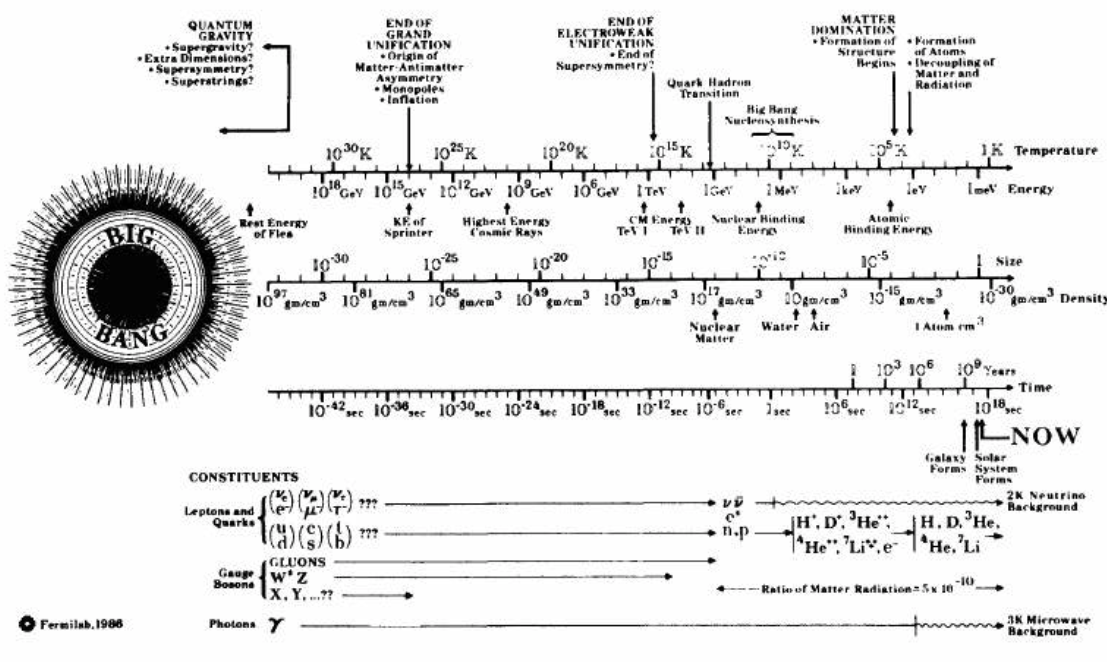
\includegraphics[width=\linewidth]{thermalhistory.png}
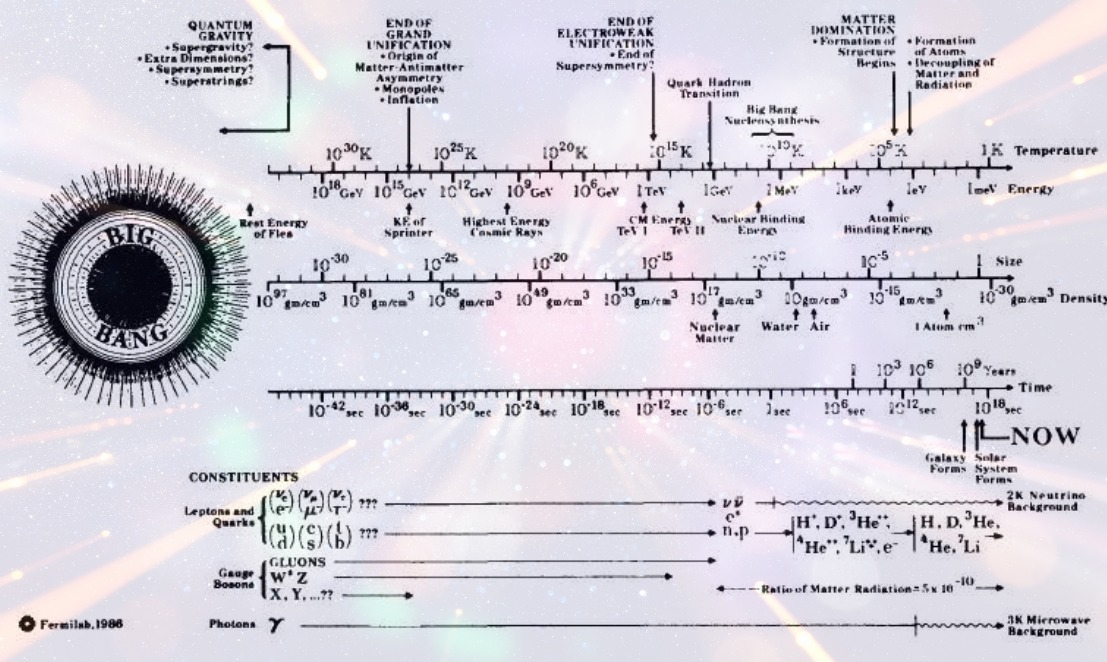
\includegraphics[width=\linewidth]{overlay.jpg}
\end{center}
\newpage
\doublespacing
\tableofcontents
\addtocontents{toc}{~\hfill\textbf{Page}\par}
\singlespacing
\renewcommand{\thefootnote}{\arabic{footnote}}
\newpage

\section{Introduction}


There are a number of recent datasets that allow us to use Cosmology as a precision tool in particle physics including the Cosmic Microwave Background \citep{Bennett:2003ba}, the Hubble expansion of galaxies \citep{Fukugita:1993hc}, and the light element abundance \citep{Danziger:1970wn}. These allow us to explore the cosmological history back to around $1 \, \textrm{MeV} \simeq 1 \, \textrm{s}$ within the $\Lambda$CDM framework, see \citet{Weinberg:1972kfs}. On the particle physics side, it is believed that two phase transitions occured during the evolution. Firstly, the electroweak phase transition is believed to occur around $T_{\mathrm{EW}} \sim 250 \, \mathrm{GeV}$. At a much lower temperature, $T_{\mathrm{QCD}} \sim 200 \, \mathrm{MeV}$, chiral symmetry breaking occurs and the quarks are confined. This latter point has cosmological implications both within the standard entropic evolution of the Universe, as well as for the theoretical axion \citep{Peccei:1977ur}.

Whilst the Standard Model and $\Lambda$CDM both present high precision accounts which have been tested to extreme levels, they also suffer from the same effective field theory paradigm. Both theories have been shown to be only an effective description of the dyanmics, although they are complementary. Observations such as the baryon asymmetry in the Universe, the presence of Dark Matter, and the fine-tuning problem that is reportedly solved by inflation \citep{Guth:1980zm} are examples of the challenges yet to be overcome. Nonetheless, progress has been made e.g. the scale invariant spectrum that is a prediction of Guth's inflationary mechanism \citep{Mukhanov:1990me} is in extremely strong agreement with measurements of the Cosmic Microwave Background (CMB) by experiments such as WMAP \citep{Bennett:2003ba} and Planck \citep{Villa:2001ss}.

The acceptance of these shortcomings renders it necessary to invent and test extensions to the standard models of particle physics and cosmology. Such extensions are abundant, but a combination of (i) particle physics experiments, (ii) precision cosmological measurements, and (iii) a theory linking the two \citep{Kolb:1990vq}, can provide constraints and clear the path forward. This work is interested in the constraints on new physics that can be derived from an understanding of the complicated, highly non-equilibrium process \citep{Ellis:1979nq} of light element formation --- \textit{Big Bang Nucleosynthesis}.


\section{Preliminaries} \label{sec:prelims}


We collect some important results surrounding the $\Lambda$CDM model and standard relativistic statistical mechanics. Firstly, the assumption that the Universe is homogenous and isotropic on large scales (greater than a few Mpc, see \citet{Fukugita:1993hc}) is encapsulated in the Friedmann-Lemaitre-Robertson-Walker metric;
\begin{equation}
\mathrm{d}s^2 = g_{\mu\nu}\mathrm{d}x^\mu \mathrm{d}x^\nu = \mathrm{d}t^2 - R^2(t) \left(\frac{\mathrm{d}r^2}{1 - kr^2} + r^2(\mathrm{d}\theta^2 + \sin^2\theta \mathrm{d}\phi^2)\right).
\end{equation}
Here $R(t)$ is the scale factor, and by making a suitable co-ordinate transformation, $k$ can be chosen to be $-1$, $0$ or $1$. The energy-momentum tensor is then required to be of perfect fluid form,
\begin{equation}
T_{\mu\nu} = p g_{\mu\nu} + (p + \rho)u_\mu u_\nu.
\end{equation}
With these definitions, the Einstein field equations reduce to the \textit{Friedmann equations},
\begin{align}
H^2 &= \left(\frac{\dot{R}}{R}\right)^2 = \frac{8\pi \rho}{3M_p^2} - \frac{k}{R^2}, \\
\frac{\ddot{R}}{R} &= -\frac{4\pi \rho}{3 M_p^2}(\rho + 3p)
\end{align}
possibly with the addition of a cosmological constant, $\Lambda$ \citep{Weinberg:1988cp}. The conservation equation for the energy-momentum tensor $T_{\mu\nu}$ that arises from the Bianchi identity gives the following,
\begin{equation}
\frac{\mathrm{d}(\rho R^3)}{\mathrm{d}R} = -3p R^2. \label{eq:cons}
\end{equation}
This final equation, knowing the equation of state $p = p(\rho)$ allows us to classify the evolution of different types of matter. For example,
\begin{itemize}
\item \textit{Matter} or \textit{Dust} has $p/\rho \sim T/m \ll 1$ which gives $\rho_{\mathrm{NR}} \propto R^{-3}$,
\item \textit{Radiation} has $p = \rho/3$ which gives an additional factor $\rho_{\mathrm{R}} \propto R^{-4}$,
\item \textit{Vacuum Energy} has $p = -\rho$ leading to a constant energy density $\rho_{\mathrm{V}} \propto \mathrm{const.}$.
\end{itemize}
At any given time, $t$, the total energy density of the Universe can be compared to the \textit{critical density},
\begin{equation}
\rho_c(t) = \frac{3H^2(t)M_p^2}{8\pi}
\end{equation}
If the total energy density $\rho(t) > \rho_c(t)$, then the Universe is overdense and has $k = +1$, and similarly for $k=0, -1$. Using the fact that the radiation today is dominated by that from the CMB, and defining $\Theta = T_0/2.73 \, \mathrm{K}$\footnote{
In natural units where $\hbar = c = k_B = 1$, we have the following conversions;
\begin{align*}
&1 \, \mathrm{GeV}^{-1} = 1.973 \times 10^{-14}\,\mathrm{cm} = 6.582 \times 10^{-25} \, \mathrm{s} \\
&1 \, \mathrm{GeV} = 1.160 \times 10^{13} \, \mathrm{K} \\
&1 \, \mathrm{Mpc} = 3.086 \times 10^{24} \, \mathrm{cm}
\end{align*}
}, one can deduce,
\begin{equation}
\rho_{\gamma 0} = \frac{\pi^2 T_0^4}{15} = 2.02 \times 10^{-51} \Theta^4 \,\mathrm{GeV}^4 \Rightarrow \Omega_{\gamma 0} = \frac{\rho_{\gamma 0}}{\rho_{c 0}} = 2.49 \times 10^{-5} \Theta^4 h^{-2}.
\end{equation}
This is enough to illustrate the fact that the Universe is currently dominated by non-relativistic particles (Matter Domination). Earlier on in the evolution, this was not necessarily the case, and the Universe would have been dominated by radiation for
\begin{equation}
R < R_{\mathrm{eq}} = 4.18 \times 10^{-5}\Theta^4(\Omega_0 h^2)^{-1} \Rightarrow z_{\mathrm{eq}} \simeq 2740.
\end{equation}
This can be converted into a bound on the temperature by assuming adiabacity in the expansion ($RT = \mathrm{const.}$). Rescaling such that $R_0 = 1$ and $T_0 = 2.73 \, \mathrm{K}$, this tells us that the Universe was radiation dominated for temperatures
\begin{equation}
T > T_{\mathrm{eq}} = 5.63 \times 10^{-9} \, \mathrm{GeV}\,(\Omega_0 h^2 \Theta^{-3}) \simeq 2.59 \times 10^{-9} \, \mathrm{GeV},
\end{equation}
where we have taken the scale factor for the Hubble expansion, $h = 0.678$. The important conclusion from this is that particle physics processes are interesting when $T > m$, where $m$ is the mass of a given particle. We see that the bound above implies that \textit{cosmological processes of interest to particle physics occur almost entirely during the radiation dominated era}.


\subsection{Equilibrium in the Early Universe}

To understand the thermal history of the Universe, we must first understand whether certain particle species are in equilibrium or not. This is determined by comparing their interaction rate, $\Gamma(T)$, with the Hubble expansion rate $H(T)$ \citep{Schramm:1977ne}. Full thermodynamic equilibrium is characterised by two processes,
\begin{enumerate}
\item \textit{Kinetic Equilibrium} --- this is established when there are sufficiently rapid elastic scattering processes to exchange energy between different particle species.
\item \textit{Chemical Equilibrium} --- this is established when there are processes which can efficiently create and remove particles.
\end{enumerate}
A couple of assumptions renders the approximation of the Early Universe as an ideal gas a good one away from phase transitions. Firstly, the particle densities are not usually high enough for many-body interactions to become important. Secondly, the interaction strengths are broadly in the perturbative regime (in the quark sector, this is ensured by the asymptotic freedom of the strong interaction). For $2 \rightarrow 2$ processes at very high temperatures, on dimensional grounds $\sigma \propto T^{-2} \Rightarrow \Gamma(T) = n(T)\langle \sigma v \rangle \propto T$, but the Hubble rate, $H(T) \propto T^2$. This leads to a maximum temperature\footnote{This maximum temperature is derived assuming that initially the Universe starts as a cold gas at the Planck scale.} above which kinetic equilibrium is attained of $\simeq 3 \times 10^{14}\,\mathrm{GeV}$ \citep{Elmfors:1993pz}. Similar considerations ascertain that $2 \rightarrow 3$ processes lead to a chemical equilibrium being attained at temperatures around $10^{12}\,\mathrm{GeV}$.

\subsection{Statistical Physics Preliminaries}


For a quantum ideal gas, the \textit{equilibirum phase space density}, $f^{\mathrm{eq}}_i(q, T)$ is given by,
\begin{align}
f_B^{\mathrm{eq}}(q, T) &= \left[\exp\left(\frac{E_i - \mu_i}{T}\right) - 1\right]^{-1} \quad \mathrm{(Bose \,\, Statistics)} \\
f_F^{\mathrm{eq}}(q, T) &= \left[\exp\left(\frac{E_i - \mu_i}{T}\right) + 1\right]^{-1} \quad \mathrm{(Fermi \,\, Statistics)}
\end{align}
The chemical potentials $\mu_i$ for gauge bosons such as photons and $Z^0$ bosons is zero ($\mu_\gamma = \mu_Z = 0$) since they can be emitted or absorbed at high enough temperatures.\footnote{This is not necessasrily true for $W$ bosons and gluons as they carry non-trivial quantum numbers. We \textit{assume} that the Universe has no net colour or hypercharge.} See \citet{Haber:1981fg} for a discussion of the interpretation of this ultra-relativistic gas and the chemical potential in quantum field theory. The net electric charge of the Universe, as well as the net baryon to photon ratio, $\eta = (N_B + N_{\bar{B}})/N_\gamma \sim 10^{-9}$ are both empirically very small \citep{Steigman:1979kw}. This ensures that in most situations, for simplicity, it is reasonable to set $\mu_e = \mu_B = 0$. A similar conclusion regarding the lepton number vs. the photon number leads people to make the assumption that $\mu_\nu = 0$ also, although this can be relaxed later. This is particularly relevant if the baryon number minus the lepton number ($B - L$) is large. In this case there will be a large chemical potential in neutrinos which can affect Big Bang Nucleosynthesis.

We can now collect the standard thermodynamic variables for an \textit{equilibrium} Bose or Fermi gas at zero chemical potential;
\begin{align}
n_i^{\mathrm{eq}} &= g_i \int{\frac{\mathrm{d}^3 q}{(2\pi)^3} \, f_i^{\mathrm{eq}}(q, T)} = \frac{g_i}{2\pi^2}T^3 I_{i}^{11}(\mp), \label{eq:neq}\\
\rho_i^{\mathrm{eq}} &= g_i \int{\frac{\mathrm{d}^3 q}{(2\pi)^3} \, E_i(q) f_i^{\mathrm{eq}}(q, T)} = \frac{g_i}{2\pi^2}T^4 I_{i}^{21}(\mp), \label{eq:req}\\
p_i^{\mathrm{eq}} &= g_i \int{\frac{\mathrm{d}^3 q}{(2\pi)^3} \, \frac{q^2}{3E_i(q)}f_i^{\mathrm{eq}}(q, T)} = \frac{g_i}{6\pi^2}T^4 I_{i}^{03}(\mp), \label{eq:peq}
\end{align}
where,
\begin{equation}
I_i^{mn}(\mp) = \int_{x_i}^{\infty}{\mathrm{d}y\,\frac{y^m(y^2 - x_i^2)^{n/2}}{e^y \mp 1}}, \quad x_i = \frac{m_i}{T}.
\end{equation}
These relations also give the second law of thermodynamics \citep{Weinberg:1972kfs},
\begin{equation}
\frac{\mathrm{d}p^{\mathrm{eq}}}{\mathrm{d}T} = \frac{(\rho^{\mathrm{eq}} + p^{\mathrm{eq}})}{T}.
\end{equation}
There are two regimes where we can extract some analytic expressions for these quantities;
\begin{enumerate}
\item \textit{Relativistic Particles} --- if $T \gg m_i \Leftrightarrow x_i \ll 1$, then the integrals $I^{mn}(T)(\mp)$ reduce to the Riemann zeta function integral representation,
\begin{equation}
\zeta(n) = \frac{1}{\Gamma(n)}\int_{0}^{\infty}{\mathrm{d}y \, \frac{y^{n - 1}}{e^y - 1}}
\end{equation}
For bosons, this gives,
\begin{equation}
I_R^{11}(-) = 2\zeta(3), \quad I_R^{21}(-) = I_R^{03}(-) = \frac{\pi^4}{15},
\end{equation}
whilst for fermions, we find,
\begin{equation}
I_R^{11}(+) = \frac{3\zeta(3)}{2}, I_R^{21}(+) = I_R^{03}(+) = \frac{7\pi^4}{120}.
\end{equation}
This allows us to write the number and energy densities as,
\begin{equation}
n_i^{\mathrm{eq}}(T) = \frac{g_i \zeta(3)}{\pi^2} T^3 \times \begin{cases} 1 & \mathrm{(Bosons)}\\ \frac{3}{4} & \mathrm{(Fermions)}\end{cases}, \quad \rho_i^{\mathrm{eq}}(T) = \frac{g_i \pi^2}{30} T^4 \times \begin{cases} 1 & \mathrm{(Bosons)}\\ \frac{7}{8} & \mathrm{(Fermions)}\end{cases}
\end{equation}
The pressure is then given by $p_i^{\mathrm{eq}}(T) = \rho_i^{\mathrm{eq}}(T)/3$.
\item \textit{Non-relativistic particles} --- if $T \ll m_i \Leftrightarrow x_i \gg 1$, then we can approximate,
\begin{equation}
I^{mn}(\mp) \simeq \int_{0}^{\infty}{\mathrm{d}y \, y^2 \exp\left(-\sqrt{y^2 + x_i^2}\right)}
\end{equation}
This is dominated by the contribution around $y = 0$, so we can expand $\sqrt{y^2 + x_i^2} = x_i(1 + y^2/2x_i^2 + \cdots)$ and then perform the integration by completing the square. We find,
\begin{equation}
I^{mn}(\mp) \simeq \int_0^{\infty}{\mathrm{d}y \, y^2 e^{-x_i}e^{-y^2/2x_i}}
\end{equation}
If we further note that $E_i(q) \simeq m$ for non-relativistic particles, then then integral for $\rho_i^{\mathrm{eq}}$ reduces to $m n_i^{\mathrm{eq}}$. Then we can write the number and energy densities in the non-relativistic cases as (we include the case of a non-zero chemical potential in this scenario),
\begin{equation}
n_i^{\mathrm{eq}}(T) = g_i\left(\frac{m_iT}{2\pi}\right)^{3/2} e^{-m_i/T}e^{\mu_i/T}, \quad \rho_i^{\mathrm{eq}}(T) = m_i n_i^{\mathrm{eq}}(T), \quad p_i^{\mathrm{eq}}(T) \simeq 0.
\end{equation}
It is important to note that the Boltzmann distribution is not invariant under the cosmic expansion, so non-relativistic particles only stay in equilibrium if they interact rapidly with a dominant population of relativistic particles\footnote{See pp.14-15 of \citet{Bernstein:1988bw} and the discussion of the Liouville operator, $L$, in a flat FLRW Universe. The statement that the shape of the distribution remains unchanged by the expansion is equivalent to the Bose and Fermi distributions being solutions to the collisionless Boltzmann equation $L(f) = 0$.}. The evolution of the number and energy densities is shown in Figure \ref{fig:nandrho} for electrons and photons. We see the Boltzmann suppression takes hold below the electron mass.
\end{enumerate}
Outside of these two regimes, the integrals must be done numerically. The results of this are shown in Figure \ref{fig:idealgas}, where we can see the behaviour of the equation of state $p = p(\rho)$ and the Boltzmann suppression in the non-relativistic case.
\begin{figure}[t]
\begin{center}
\includegraphics[width=\linewidth]{IdealGas.pdf}
\caption{The behaviour of $n_i^{\mathrm{eq}}$, $\rho_i^{\mathrm{eq}}$, and the equation of state $p_i^{\mathrm{eq}}/\rho_i^{\mathrm{eq}}$ as a function of $x_i = m_i/T$.}\label{fig:idealgas}
\end{center}
\end{figure}
\begin{figure}[t]
\begin{center}
\includegraphics[width=\linewidth]{NandRho.pdf}
\caption{The behaviour of $n^{\mathrm{eq}}(T)$ and $\rho^{\mathrm{eq}}(T)$ as a function of the temperature in the case of electrons and photons. We see that for electrons, there is the predicted Boltzmann suppression below the electron mass.}\label{fig:nandrho}
\end{center}
\end{figure}
Now, when all the particles present are in equilibrium, we can compute the total number of relativistic degrees of freedom, $g_R$, via;
\begin{equation}
g_R = \sum_{B}{g_i} + \frac{7}{8}\sum_{F}{g_i}.
\end{equation}
The introduction of the non-relativistic degrees of freedom leads to $\sim 10 \%$ correction. It is not in general true that at a given time, all relativistic species will be in equilibirum. The particles will only be in kinetic equilibrium (i.e. $T_i = T$) with the background thermal plasma ($e^-$ and photons above $T = m_e$, below which Compton scattering becomes inefficient) while they are interacting.  This is equivalent to the scattering rate $\Gamma_i = n_i \langle \sigma_{\mathrm{scat}}v \rangle$ exceeding the expansion rate $H(T)$. Here $\langle \sigma_{\mathrm{scat.}}v \rangle$ is the velocity averaged cross section for $2 \rightarrow 2$ processes such as $i \gamma \rightarrow i \gamma$ or $i \ell^{\pm} \rightarrow i \ell^{\pm}$. The particle, $i$, is then said to \textit{decouple} when,
\begin{equation}
\Gamma_i(T_D) = H(T_D)
\end{equation}
This is of course a simplification in that there will be residual interactions, but these are negligble for a first order approximation to e.g. neutrino decoupling \citep{Dodelson:1992km}. For \textit{relativistic} particles, we can break up the process as follows,
\begin{enumerate}
\item If the particle is relativistic at $T_D$ (which in practice is only true for neutrinos in the Standard Model, which are very light and weakly coupled), then it will also be in chemical equilibrium with the thermal plasma. This is attained via processes such as $i \bar{i} \rightarrow \gamma \gamma, \ell^+ \ell^-$. In this case, the abundance at decoupling will just be the thermodynamic equilibrium (equiv. kinetic + chemical equilibrium) value, $n_i^{eq}(T_D)$ as given by equation \eqref{eq:neq}.
\item After decoupling, \textit{as long as the particle remains relativistic}, the phase space distribution will continue to be of the equilibrium form, with $T_i$ replacing $T$. In this case, $T_i, E_i \propto R^{-1}$.
\item Up until the point where other massive standard model particles annihilate into photons and other interacting species, the temperature $T_i$ will track the photon temperature $T$.
\item After the annihilation however, the photons and other interacting species will be heated and the temperature of the thermal plasma will exceed that of the particles $i$; $T > T_i$.
\item This will cause the number density of particle $i$ relative to the photons to drop (ultimately we have just generated more photons in the annihilation) i.e. $n_i/n_\gamma$ will drop below its value at decoupling, $n_i(T_D)/n_\gamma(T_D)$.
\end{enumerate}
To compute this ratio, we broadly follow the classic text in \citet{Alpher:1953zz}. To start, we split the total energy density and pressure into \textit{interacting} (I) and \textit{decoupled} (D) parts. Importantly, the interacting part is a function of the temperature of the thermal bath, $T$, whilst the decoupled part depends only on the scale factor, $R$, and the decoupling temperature, $T_D$,
\begin{equation}
p = p_I(T) + p_D(R; T_D), \quad \rho = \rho_I(T) + \rho_D(R; T_D)
\end{equation}
We can also write the conervation equation in \eqref{eq:cons} as,
\begin{equation}
R^3 \frac{\mathrm{d}p}{\mathrm{d}T} = \frac{\mathrm{d}}{\mathrm{d}T}\left[R^3 (\rho + p)\right]
\end{equation}
If we assume that the decoupled particles eventually become non-relativistic, then applying conservation of number density $n_D R^3 = \mathrm{const.}$ is equivalent to conserving energy density. Hence,
\begin{equation}
R^3\frac{\mathrm{d}\rho_D}{\mathrm{d}R} \frac{\mathrm{d}R}{\mathrm{d}T} + 3R^2 \frac{\mathrm{d}R}{\mathrm{d}T}\rho_D = 0.
\end{equation}
If we also neglect the pressure, $p_D = 0$, for the non-relativistic decoupled particles, then the conservation equation reduces to,
\begin{equation}
\frac{\mathrm{d}\log R}{\mathrm{d}\log T} = -\frac{1}{3}\frac{1}{\rho_I + p_I}\frac{\mathrm{d}\rho_I}{\mathrm{d}\log T}
\end{equation}
We can use the second law of thermodynamics for $\rho_I$ and $p_I$ to show that this is equivalent to,
\begin{equation}
\frac{\mathrm{d}\log R}{\mathrm{d}\log T} = -1 - \frac{1}{3}\frac{\mathrm{d}\log\left(\frac{\rho_I + p_I}{T^4}\right)}{\mathrm{d}\log T}. \label{eq:specifcentropy}
\end{equation}
This can be integrated to give;
\begin{equation}
\log R = - \log T - \frac{1}{3}\log \left(\frac{\rho_I + p_I}{T^4}\right) + \mathrm{const.}
\end{equation}
Note that if $\rho_I + p_I \propto T^4$ as is the case for a gas of blackbody photons then we obtain the \textit{adiabatic invariant}, $RT = \mathrm{const.}$. The second term accounts for non-adiabacity due to changes in the number of interacting species.

Importantly we can now compare different epochs with different numbers of interacting species. These are related by noting that \eqref{eq:specifcentropy} is equivalent to conservation of the \textit{specific entropy}, $S_I = s_I R^3$ in the sense that $\mathrm{d}S_I/\mathrm{d}T = 0$. Here,
\begin{equation}
s_I \equiv \frac{\rho_I + p_I}{T} = \sum_{I}{\frac{\rho_i + p_i}{T}},
\end{equation}
i.e. a sum over all interacting species in equilibrium. Using \eqref{eq:neq} --- \eqref{eq:peq}, this is equivalent to calculating,
\begin{equation}
s_i(T) = g_i \int{\frac{\mathrm{d}^3q}{(2\pi)^3}\,f_i^{\mathrm{eq}}(q, T) \frac{3m_i^2 + 4q^2}{3E_i(q) T}}
\end{equation}
A convenient way to parametrise this, and the energy density is via,
\begin{equation}
s_i(T) \equiv \left(\frac{g_{s_i}(T)}{2}\right)\left(\frac{4}{3}\frac{\rho_\gamma(T)}{T}\right), \quad \rho_i^{\mathrm{eq}}(T) \equiv \left(\frac{g_{\rho_i}(T)}{2}\right)\rho_\gamma.
\end{equation}
Using the fact that $\rho_\gamma(T) = \pi^2 T^4/15$, and for radiation $s = 4\rho/3$, we see this is normalised to the photon distribution. Finally, using the thermodynamics definitions, we find that,
\begin{equation}
g_{s_i}(T) = \frac{45}{4\pi^4}g_i \left[I_i^{21}(m/T; \mp) + \frac{1}{3}I_i^{03}(m/T; \mp)\right], \quad g_{\rho_i}(T) = \frac{15}{\pi^4}g_i I_i^{21}(m/T; \mp)
\end{equation}
This again reiterates the fact that non-relativistic species contribute little to the effective degrees of freedom in the plasma. The number of \textit{interacting} degrees of freedom (c.f. $g_R$ as the number of \textit{relativistic} degrees of freedom) is then given by;
\begin{equation}
g_{s_I} = \sum_{I}{g_{s_i}},
\end{equation}
which is a sum over all species which are interacting with the plasma.
\subsection{Temperature of Decoupled Species}
Suppose a particle, $j$, decouples from the thermal plasma at $T_D$, then we want to calculate how the temperature $T_j$ compares to the photon temperature $T$. To do so, we note that for $T < T_D$, the entropy of the decoupled particles and the entropy of the still interacting particles is separately conserved. Then,
\begin{align*}
S - S_I = s_j R^3 &= \frac{2\pi^2}{45}g_{s_j}(T) (RT_j)^3 \\
S_I = \sum_{I}{s_i(T)R^3} &= \frac{2\pi^2}{45}g_{s_I}(T)(RT)^3
\end{align*}
can be compared at decoupling and again at a lower temperature. This gives the following relations,
\begin{align*}
g_{s_j}(T_D) R_D^3 T_D^3 &= g_{s_j}(T) R^3 T_j^3, \\
g_{s_I}(T_D) R_D^3 T_D^3 &= g_{s_I}(T) R^3 T^3.
\end{align*}
Dividing the two results gives the result \citep{Srednicki:1988ce},
\begin{equation}\label{eq:tnutg}
\frac{T_j}{T} = \left[\frac{g_{s_j}(T_D)}{g_{s_j}(T)}\frac{g_{s_I}(T)}{g_{s_I}(T_D)}\right]^{1/3}
\end{equation}
This accounts for the fact that entropy can be injected into the decoupled sector (for example annihilation into neutrinos) changing the value of $g_{s_j}$ at decoupling. This also allows to understand what happens when a particle becomes non-relativistic and annihilates into the other relativistic particles. The degrees of freedom that specify the total conserved entropy is given by,
\begin{equation}
g_s(T) = g_{s_I}(T)\left[1 + \frac{g_{s_j}(T_D)}{g_{s_I}(T_D)}\right]
\end{equation}
Now we see that if particle $j$ becomes non-relativistic, then $g_{s_j}(T_D) \simeq 0$ and $g_s$ reflects simply all relativistic interacting species at temperature $T$. On the other hand, if the decoupled species is relativistic, as is the case with neutrinos, then $g_s$ includes the contribution of these particles, weighted by the temperature difference. This allows us to define the parameter,
\begin{align}
g_{\star S}(T) &= \sum_{I}{g_{s_i}(T)} + g_{s_j}(T_j)\left(\frac{T_j}{T}\right)^3, \\
&\simeq \sum_{B}{g_i\left(\frac{T_i}{T}\right)^3} + \frac{7}{8}\sum_{F}{g_i\left(\frac{T_i}{T}\right)^3}.
\end{align}
The last equation holds when all the particles are \textit{relativistic}. We have a similar expression for the effective number of relativistic degrees of freedom,
\begin{equation}
g_\rho(T) \simeq \sum_{B}{g_i\left(\frac{T_i}{T}\right)^4} + \frac{7}{8}\sum_{F}{g_i\left(\frac{T_i}{T}\right)^4}. \label{eq:grho}
\end{equation}
\subsection{Example: Neutrino Decoupling in the Standard Model}
We will illustrate these ideas with a simplified version of neutrino decoupling in the standard model. If we take the thermally averaged cross section to be $\langle \sigma v \rangle \sim G_F^2 T^2$, then the interaction rate is $\Gamma \sim G_F^2 T^5$. In radiation domination, a useful relation between the Hubble rate, $H$, and the temperature, $T$, is given by;
\begin{equation}
H = 1.66 \, g_\rho^{1/2}\frac{T^2}{M_p}
\end{equation}
This let's us deduce that the expansion rate $H \sim \Gamma$ at a decoupling temperature of\footnote{A more careful analysis \citep{Dicus:1982cb} gives $T_D(\nu_\mu, \nu_\tau) = 3.5 \, \mathrm{MeV}$ and $T_D(\nu_e) = 2.3 \, \mathrm{MeV}$},
\begin{equation}
T_D(\nu) \sim (G_F^2 M_p)^{-1/3} \sim 1\,\mathrm{MeV}
\end{equation}
Now, above this temperature, the number densities in photons and neutrinos satisfy $n_\nu^{\mathrm{eq}} = (3/4)n_\gamma^{\mathrm{eq}}$. After decoupling at $1 \, \mathrm{MeV}$, the electrons and positrons annihilate (at temperatures around $500 \, \mathrm{keV}$). The ensures that the number of interacting degrees of freedom decreases from $11/2$ (photons + $e^{\pm}$) to $2$ (photons). This allows us to compute the ratio of neutrino temperature to photon temperature through the period of $e^{\pm}$ annihilation,
\begin{equation}
\frac{T_\nu}{T} = \left(\frac{4}{11}\right)^{1/3}\left[1 + \frac{45}{2\pi^4}\left(I^{21}(m_e/T; +) + \frac{1}{3}I^{03}(m_e/T; +)\right)\right]^{1/3} \rightarrow \left(\frac{4}{11}\right)^{1/3}
\end{equation}
We illustrate this in Figure \ref{fig:tnutg}. This assumes that the neutrino decoupling is instantaneous. In reality, this is of course not true, especially since the cross-section for the scattering of neutrinos is proportional to the energy. Hence, higher energy neutrinos will recieve more of a contribution due to electron-positron heating than lower energy neutrinos. This will have the effect of altering the spectrum away from the Fermi-Dirac equilibrium statistics. The implementation of this with the Boltzmann equation is done by \citet{Dodelson:1992km} and \citet{Hannestad:1995rs}. This also lets us define the number of effective cosmological neutrinos, $N_{\mathrm{eff}}$ via,
\begin{equation}
\rho_R = \left[1 + \frac{7}{8}\left(\frac{4}{11}\right)^{4/3}N_{\mathrm{eff}}\right]\rho_\gamma \Rightarrow N_{\mathrm{eff}} \equiv \left(\frac{\rho_R - \rho_\gamma}{\rho_\nu^0}\right) \left(\frac{\rho_\gamma^0}{\rho_\gamma}\right).
\end{equation}
In the Standard Model, this is given by,
\begin{equation}
N_{\mathrm{eff}} = 3\left(\frac{11}{4}\right)^{4/3} \left(\frac{T_\nu}{T_\gamma}\right)^4
\end{equation}
This is under the assumption that only neutrinos and photons are present and that their distribution functions can be characterised by their temperature. There are departures from this which exist \textit{within} the Standard Model due to,
\begin{enumerate}
\item \textit{Thermal QED Corrections:} Due to interactions of the electrons and photons with the thermal plasma, thermal masses are generated which come into the dispersion relations.
\item \textit{Non-instantaneous Decoupling:} The calculation that we illustrated above assumed that the neutrinos decoupled instantaneously from the plasma. This is not the case in reality and instead the neutrinos do receive some temperature boost during $e^{\pm}$ annihilation. This increases the value of $N_{\mathrm{eff}}$ slightly and distorts the Fermi distribution functions.
\end{enumerate}
The combination of these lead to a Standard Model prediction of $N_{\mathrm{eff}} = 3.045$. Both these effects will be considered in greater detail in Section \ref{sec:neff}: \textit{\nameref{sec:neff}}, with a discussion based on \cite{Mangano:2001iu} and \cite{Escudero:2018mvt}. Furthermore, the impact of new physics scenarios, in particular WIMPS, will be covered in Section \ref{sec:newphys}: \textit{\nameref{sec:newphys}} where the main references are \cite{Boehm:2013jpa} and \cite{Nollett:2014lwa}.
\begin{figure}[t]
\begin{center}
\includegraphics[width=0.5\linewidth]{../Figures/TnuTg.pdf}
\caption{The ratio between the neutrino temperature and the photon temperature as the process of electron and positron annihilation proceeds once the temperature drops below the electron mass.}\label{fig:tnutg}
\end{center}
\end{figure}



\section{Primordial Nucleosynthesis}


At the time of \citet{Sarkar:1995dd}, the light element abundance was the most precise laboratory for particle physics due to the lack of development regarding CMB physics. Now, of course, the combination of the two measurements provides the most detailed and constraining physics case for new phenomelogical models. The goal of this section is to first understand the process of light element synthesis, and secondly the dependence of the final abundances on various physical parameters ($g_{\star S}, \eta, \cdots$). At the end of the day, much of the detailed analysis must be done numerically taking into account all the different nuclear reaction rates.


\subsection{The Standard BBN Model}


In this simplified analysis, we will consider the synthesis of light eleements in the early Universe as occuring in two distinct stages. This is made possible by the high entropy per nucleon in the Universe $s/n_N \sim 10^{11}$ which prefers unbound nucleons until the temperature is sufficiently low that the binding energy is the dominant term in the free energy $F = E - TS$. The two processes are as follows;
\begin{enumerate}
\item \textit{Decoupling of Weak Interactions} --- At temperatures around $1$ MeV, the weak interactions decouple (which also leads to neutrino decouplling), leading to the process that keeps protons and neutrons in equilibrium becoming inefficient\footnote{The main reference for this section is Chap. 9 in \citet{Bernstein:1988bw}.}.
\item \textit{Nuclear Reactions} --- After the neutron abundance has been built up, the nuclear reaction chain can proceed and synthesise the heavier nuclei such as Helium-4, Lithium-7 etc.  
\end{enumerate}



\subsection{Neutron Freeze-out}


At sufficiently high temperatures, neutrons, protons, electrons, neutrinos, and photons are all in kinetic equilibrium via weak and electromagnetic interactions ($T_e = T_p = T_n = T_\nu = T$)\footnote{This ceases to be true at lower temperatures when the neutrinos decouple, leading to $\sim 10 \%$ correction.}. The electrons ($e^{\mp}$), neutrinos ($\nu_e$), neutrons ($n$), and protons ($p$) are kept in equilibrium by the following processes;
\begin{align}
n + \nu_e &\rightleftharpoons p + e^{-}, \\
n + e^{+} &\rightleftharpoons p + \bar{\nu}_e, \\
n &\rightleftharpoons p + e^{-} + \bar{\nu}_e.
\end{align}
These lead to the following relationships between the chemical potentials,
\begin{equation}
\mu_n - \mu_p = \mu_{e^{-}} - \mu_{\nu_e} = \mu_{\bar{\nu}_e} - \mu_{e^{+}}.
\end{equation}
If we define,
\begin{equation}
\lambda_{np}(t) = \lambda(n \nu_e \rightarrow p e^{-}) + \lambda(n e^{+} \rightarrow p \bar{\nu}_e) + \lambda(n \rightarrow p e^{-} \bar{\nu}_e)
\end{equation}
as the total rate for the conversion of protons into neutrons, then the rate for the reverse reaction is given by the detailed balance,
\begin{equation}
\lambda_{pn}(t) = \lambda_{np}(t) e^{-\Delta m/T(t)}, \quad \Delta m \equiv m_n - m_p = 1.293 \, \mathrm{MeV}. \label{eq:rates}
\end{equation}
As this stands, we are assuming that there is not a large chemical potential in neutrinos, which would also appear in the exponential. Furthemore, one can assume that the chemical potential of electrons must be very small given that the electrical neutrality of the Universe implies $n_e \sim n_p$. Thus, $\mu_e/T \sim n_e/n_\gamma \sim n_p/n_\gamma \sim 10^{-10}$.

Now, if we define $n_N(t) = n_n(t) + n_p(t)$, and then let the fractional abundances of neutrons and protons be,
\begin{equation}
X_n(t) \equiv \frac{n_n(t)}{n_N(t)}, \quad X_p(t) \equiv \frac{n_p(t)}{n_N(t)} \quad (\Rightarrow X_n(t) + X_p(t) = 1).
\end{equation}
Then $X_n(t)$ satisfies the differential equation,
\begin{equation}
\frac{\mathrm{d}X_n(t)}{\mathrm{d}t} = \lambda_{pn}(t) X_p(t) - \lambda_{np}(t) X_n(t) = \lambda_{pn}(t)\left(1 - X_n(t)\right) - \lambda_{np}(t)X_n(t).
\end{equation}
Using the relation in \eqref{eq:rates} this can be written as,
\begin{equation}
\frac{\mathrm{d}X_n(t)}{\mathrm{d}t} = \lambda_{pn}(t) \left[ 1 - \left(1 + e^{\Delta m/T(t)}\right)X_n(t)\right] = \lambda_{pn}(t) - \Lambda(t) X_n(t),
\end{equation}
where $\Lambda(t) = \lambda_{pn}(t) + \lambda_{np}(t)$. The equilibirium solution is found by setting $\mathrm{d}X_n(t)/\mathrm{d}t = 0$, giving,
\begin{equation}
X_n^{\mathrm{eq}}(t) = \frac{\lambda_{pn}(t)}{\Lambda(t)} = \left[1 + e^{\Delta m/T(t)}\right]^{-1}.
\end{equation}
The general solution on the other hand is givne by,
\begin{align}
X_n(t) &= \int_{t_i}^{t}{\mathrm{d}t^{\prime} \, I(t, t^{\prime}) \lambda_{pn}(t^{\prime})} + I(t, t_i) X_n(t_i) \label{eq:xn}\\
I(t, t^{\prime}) &\equiv \exp\left[-\int_{t^{\prime}}^{t}{\mathrm{d}t^{\prime \prime}\,\Lambda(t^{\prime\prime})}\right]. \label{eq:It}
\end{align}
To see this is indeed a solution we note that with the definition above,
\begin{align*}
\dot{X}_n(t) &= \underbrace{I(t, t)}_{=1}\lambda_{pn}(t) + \int_{t_i}^{t}{\mathrm{d}t^{\prime} \, \frac{\mathrm{d}I(t, t^{\prime})}{\mathrm{d}t}\lambda_{pn}(t^{\prime})} + \frac{\mathrm{d}I(t, t_i)}{\mathrm{d}t}X_n(t_i) \\
\frac{\mathrm{d}I(t, t^{\prime})}{\mathrm{d}t} &= \exp\left[-\int_{t^{\prime}}^{t}{\mathrm{d}t^{\prime\prime}\,\Lambda(t^{\prime\prime})}\right] \times \left(-\Lambda(t)\right) \\
&= -\Lambda(t) I(t, t^{\prime}) \\
\Rightarrow \dot{X}_n(t) &= \lambda_{pn}(t) - \int_{t_i}^{t}{\mathrm{d}t^{\prime}\,\Lambda(t)\lambda_{pn}(t^{\prime}) I(t, t^{\prime})} - \Lambda(t)I(t, t_i)X_n(t, t_i) \\
&= \lambda_{pn}(t) - \Lambda(t)X_n(t)
\end{align*}
The important observation to make from Equations \eqref{eq:xn} and \eqref{eq:It} is the insensitivity of $X_n(t)$ to the initial condition $X_n(t_i)$. If $t$ is suitably large, then $I(t, t_i)$ is very suppressed due to the high rates, $\lambda_{np}$ and $\lambda_{pn}$ in the early Universe. As such, it is a good approximation to take $t_i = 0$ and neglect the second term in \eqref{eq:xn},
\begin{equation}
X_{\mathrm{n}}(t)=\int_{0}^{t} \mathrm{d} t^{\prime} I\left(t, t^{\prime}\right) \lambda_{\mathrm{pn}}\left(t^{\prime}\right)
\end{equation}
Integrating by parts and using the fact that $\mathrm{d}I(t, t^{\prime})/\mathrm{d}t^{\prime} = \Lambda(t)I(t, t^{\prime})$, this simplifies to
\begin{align*}
X_n(t) &= \int_{0}^{t}{\mathrm{d}t^{\prime} \, \Lambda(t^{\prime}) I(t, t^{\prime}) \frac{\lambda_{pn}(t^{\prime})}{\Lambda(t^{\prime})}}, \\
&= \int_0^{t}{\mathrm{d}t^{\prime}\, \frac{\mathrm{d}}{\mathrm{d}t^{\prime}}\left[I(t, t^{\prime})\right] \frac{\lambda_{pn}(t^{\prime})}{\Lambda(t^{\prime})}}, \\
&= \left[I(t, t^{\prime}) \frac{\lambda_{pn}(t^{\prime})}{\Lambda(t^{\prime})}\right]_{t^{\prime} = 0}^{t^{\prime} = t} -\int_{0}^{t} \mathrm{d} t^{\prime}\, I\left(t, t^{\prime}\right) \frac{\mathrm{d}}{\mathrm{d} t^{\prime}}\left[\frac{\lambda_{\mathrm{pn}}\left(t^{\prime}\right)}{\Lambda\left(t^{\prime}\right)}\right], \\
&= \frac{\lambda_{\mathrm{pn}}(t)}{\Lambda(t)}-\int_{0}^{t} \mathrm{d} t^{\prime}\, I\left(t, t^{\prime}\right) \frac{\mathrm{d}}{\mathrm{d} t^{\prime}}\left[\frac{\lambda_{\mathrm{pn}}\left(t^{\prime}\right)}{\Lambda\left(t^{\prime}\right)}\right],
\end{align*}
where we have used $I(t, 0) \sim 0$ and $I(t, t) = 1$. Integrating by parts again using the same manipulation, we find,
\begin{equation}
X_n(t) \simeq X_n^{\mathrm{eq}}(t) - \left[I(t, t^{\prime}) \frac{1}{\Lambda(t^{\prime})} \frac{\mathrm{d}}{\mathrm{d}t^{\prime}}\left(\frac{\lambda_{pn}(t^{\prime})}{\Lambda(t^{\prime})}\right)\right]^{t}_{0} + \int_{0}^{t}{\mathrm{d}t^{\prime}\,I(t, t^{\prime}) \frac{\mathrm{d}}{\mathrm{d}t^{\prime}}\left(\frac{1}{\Lambda(t^{\prime})} \frac{\mathrm{d}}{\mathrm{d}t^{\prime}}\left[\frac{\lambda_{pn}(t^{\prime})}{\Lambda(t^{\prime})}\right]\right)}.
\end{equation}
We can view this as a correction to the equilibrium value, and in the regime where the total rate is large compared to the time variation in the individual rates, we can neglect the second term,
\begin{align*}
X_n(t) &\simeq \frac{\lambda_{pn}(t)}{\Lambda(t)} - \frac{1}{\Lambda(t)} \frac{\mathrm{d}}{\mathrm{d}t}\left[\frac{\lambda_{pn}(t)}{\Lambda(t)}\right] \\
&= X_n^{\mathrm{eq}}\left[1 - \frac{1}{\Lambda(t)} \frac{\mathrm{d}\log X_n^{\mathrm{eq}}}{\mathrm{d}t}\right] \\
&= X_n^{\mathrm{eq}}\left[1 - \frac{1}{\Lambda(t)} \frac{\dot{T}}{T}\frac{\mathrm{d}\log X_n^{\mathrm{eq}}}{\mathrm{d} \log T}\right].
\end{align*}
In this regime, away from phase transitions, $RT = \mathrm{const.} \Rightarrow \dot{R}/R = -\dot{T}/T$ so we can write this as,
\begin{equation}
X_n(t) \simeq X_n^{\mathrm{eq}}\left[1 + \frac{H(t)}{\Lambda(t)} \frac{\mathrm{d}\log X_n^{\mathrm{eq}}}{\mathrm{d} \log T}\right].
\end{equation}
This last form gives us the intution that there are two regimes of interest,
\begin{enumerate}
\item $\Lambda(t) \gg H(t)$ --- when the interaction rate is much higher than the expansion rate, the neutron abundance tracks its equilibrium abundance, $X_n^{\mathrm{eq}}(t)$ as kinetic and chemical equilibrium is maintained.
\item $\Lambda(t) \ll H(t)$ --- now the second term dominates and the neutron abundance \textit{freezes out} to some non-zero, non-equilibrium value.
\end{enumerate}
To estimate the temperature at which this transition takes place, we set $\Lambda(T) \sim H(T)$ and use the following approximate expressions which are valid in the radiation domination era\footnote{These follow from $\rho = \pi^2 T^4 g_{\rho}/30$, pp.110 \citet{Bernstein:1988bw}},
\begin{equation}
H=\sqrt{\frac{8 \pi \rho}{3 M_{\mathrm{P}}^{2}}}=1.66 \, g_{\rho}^{1 / 2} \frac{T^{2}}{M_{\mathrm{P}}}, \quad t=\left(\frac{3 M_{\mathrm{P}}^{2}}{32 \pi \rho}\right)^{1 / 2}=2.42 \, g_{\rho}^{-1 / 2}\left(\frac{T}{\mathrm{MeV}}\right)^{-2} \mathrm{sec}, \label{eq:Ht}
\end{equation}
where $g_{\rho}(T)$ is as given in \eqref{eq:grho}. If we then take $\Lambda \sim n_\nu \langle \sigma v \rangle \sim G_F^2 T^5$, then $\Lambda \sim H$ gives a freeze out temperature,
\begin{equation}
T_f \sim \left(\frac{g^{1/2}_\rho}{G_F^2 M_P}\right)^{1/3}
\end{equation}
Before $e^+ e^-$ annilation, $g_\rho = g_\gamma + (7/8)[g_{e^+} + g_{e^-} + 3 g_{\nu}] = 10.75$, $G_F \sim 10^{-5} \, \mathrm{GeV}^{-2}$, and $M_P \sim 10^{19} \, \mathrm{GeV}$. So $T_f \sim g_\rho^{1/6} \times (1 \, \mathrm{MeV})$. In the Standard Model, this gives a decoupling temperature of $T_f \sim 1\, \mathrm{MeV}$. Using the second expression in \eqref{eq:Ht}, this occurs around $t \sim 1 \, \mathrm{sec}$. The neutron abundance at freeze out time is then approximately its equilibrium value,
\begin{equation}
X_n(T_f) \simeq X_n^{\mathrm{eq}}(T_f) = \left[1 + \exp\left(\frac{\Delta m}{T_f}\right)\right]^{-1} = \left[1 + \exp \left(\frac{\Delta m \cdot G_F^{2/3} \cdot  M_P^{1/3}}{g_\rho^{1/6}}\right)\right]^{-1},
\end{equation}
where in the final expression we have put in the explicit scaling of $T_f$. This is so as to indicate the effect of the different physics on the final neutron abundance, which ultimately governs the light element abundances.
\begin{itemize}
\item $\Delta m$ --- A \textit{larger} mass difference between the proton and the neutron, $\Delta m = m_n - m_p$ would lead to a \textit{lower} final neutron abundance as the equilibrium will lie further to the proton side at freeze-out. It will \textit{not} affect the freeze-out temperature.
\item $G_F$ --- A \textit{larger} value of $G_F$ i.e. if the weak interaction were stronger would lead to a lower freeze-out temperature below which the neutrons and protons fall out of equilibrium. This would result in a \textit{lower} final neutron abundance.
\item $g_\rho$ --- \textit{More} light relativistic species in the early Universe would lead to an increased expansion rate, $H$. In turn this would lead to a higher freeze-out temperature which implies a \textit{larger} final neutron abundance.
\item $M_P \propto G^{-1/2}$ --- A \textit{larger} gravitational field strength has a similar effect to increasing the number of degrees of freedom, leading to a faster expansion rate, a higher freeze-out temperature and subsequently a \textit{larger} final neutron abundance.
\end{itemize}
Note that a wide variety of different physical scales lead to this balance. The neutron-proton mass difference is governed by the strong interaction, $G_F$ by the scale of the weak interaction, and $M_P$ by the graviational force. With $\Delta m \simeq 1.293 \, \mathrm{MeV}$ and $T_f \sim 1 \, \mathrm{MeV}$ this would give a neutron abundance at freeze-out of\footnote{The exact value is of course exponentially sensitive to $\Delta m$ and $T_f$, so this value should only be taken as illustrative of the fact that a non-negligible amount of neutrons are left over.},
\begin{equation}
X_n(T_f) \simeq 0.215
\end{equation}


\subsection{Reaction Rates and the Neutron Lifetime}


In order to explicitly calculate the asymptotic neutron abundance $X_n(t \rightarrow \infty)$, the rates in $\lambda_{np}$ must be calculated exactly. These are given in \citet{Weinberg:1972kfs}\footnote{pp.547} as the following,
\begin{align}
\lambda(n\nu_e \rightarrow p e^{-}) &= A \int_{0}^{\infty}{\mathrm{d}q_\nu \, q_\nu^2 q_e E_e (1 - f_e)f_\nu}, \quad E_e = E_\nu + \Delta m \\
\lambda(n e^+ \rightarrow p \bar{\nu}_e) &= A \int_{0}^{\infty}{\mathrm{d}q_e \, q_e^2 q_\nu E_\nu (1 - f_\nu)f_e}, \quad E_\nu = E_e + \Delta m \\
\tau_n^{-1} = \lambda(n \rightarrow p e^{-} \bar{\nu}_e) &= A \int_{0}^{q_0}{\mathrm{d}q_e \, q_e^2 q_\nu E_\nu (1 - f_\nu)(1 - f_e)}, \quad q_0 = \sqrt{(\Delta m)^2 - m_e^2} \label{eq:tn}
\end{align}
Here, $f_e$ and $f_\nu$ are the Fermi-Dirac/Bose-Einstein distributions for the electrons and neutrinos,
\begin{equation}
f_e(q_e, T_e) = \left[1 + \exp\left(\frac{\sqrt{q_e^2 + m_e^2}}{T_e}\right)\right]^{-1}, \quad f_\nu = \left[1 + \exp\left(\frac{q_\nu}{T_\nu}\right)\right]^{-1}
\end{equation}
where we have allowed for the fact that the neutrinos and electrons may have (and will have after $e^{+} e^{-}$ annihilation) different temperatures. Here, the constant $A$ is dependent on strong interaction physics, where the ratio between the axial and vector couplings $G_{A}$ and $G_V$ differs from unity.\footnote{These calculations follow from the ``V-A'' theory of weak interactions.} Ultimately $A$ can be parametrised in terms of $G_A/G_V$ which can be measured experimentally, but in practice it is best to parametrise $A$ in terms of the neutron lifetime $\tau_n$ as in \eqref{eq:tn}. We will make this explicit shortly.

Now, below the neutron freeze-out temperature, $T$ ($= T_e = T_\nu$ here) is small compared to the energies of the particles (since it is below the rest mass) and the mass difference $\Delta m \sim 1.293 \, \mathrm{MeV}$. In this regime, we can replace the relativistic distributions by their Boltzmann equivalents,
\begin{equation}
f_e \simeq \exp\left(-\frac{E_e}{T_e}\right), \quad f_\nu \simeq \exp\left(-\frac{E_\nu}{T_\nu}\right).
\end{equation}
Furthermore, as a first approximation, we set the factors $1 - f_{\nu, e} \simeq 1$ since the Boltzmann factors are small in this regime. We also set $T_\nu = T_e = T$ as discussed above. The final approximation to be made is setting $m_e = 0$. To summarise these assumptions, we have taken,
\begin{enumerate}
\item The neutrino temperature to be the same as the electron temperature, $T_\nu = T_e = T$. This leads to approximately a $10 \%$ correction since after $e^{+} e^{-}$ annihilation, the electrons and positrons remain in thermal equilibrium with the photons, whilst the neutrinos have decoupled and so do not get heated.
\item Assumed that $E_{e, \nu} \gg T$ in this regime, this resulted in the distributions being replaced by their Boltzmann equivalents and the Pauli suppression $1 - f_{e, \nu} \simeq 1$.
\item Taken the electron mass to be zero, $m_e = 0$. This is justified on the premise that the contribution to the integrals near the freeze-out temperature come from a region $q \gg m_e$.
\end{enumerate}
With these simplifications in mind, the first two of the rates can be written as,
\begin{align}
\lambda(n \nu_e \rightarrow p e^{-}) &= A \int_0^{\infty}{\mathrm{d}q_\nu q_\nu^2 \left(q_\nu + \Delta m\right)^2 \exp \left(-\frac{q_\nu}{T}\right)}, \\
\lambda(n e^+ \rightarrow p \bar{\nu}_e) &= A \int_0^{\infty}{\mathrm{d}q_e q_e^2 \left(q_e + \Delta m\right)^2 \exp \left(-\frac{q_e}{T}\right)}, \\
\end{align}
which we note are identical in this case and are given by a number of $\Gamma$-function integrations. These yield,
\begin{equation}
\lambda(n \nu_e \rightarrow p e^-) = \lambda(n e^+ \rightarrow p \bar{\nu}_e) = A T^3 \left[24 \, T^2 + 12 \, T \Delta m + 2 (\Delta m)^2\right].
\end{equation}
The neutron decay rate can be computed similarly using $E_\nu + E_e= \Delta m$ as\footnote{We choose not to ignore $m_e$ here because the calculation can still be done analytically.},
\begin{equation}
\tau_n^{-1} = A \int_0^{q_0}{\mathrm{d}q_e \, q_e^2 \left(\Delta m - \sqrt{q_e^2 - m_e^2}\right)^2}.
\end{equation}
Performing the integration with the definition of $q_0$ in \eqref{eq:tn}, the neutron lifetime is given by\footnote{Setting instead $m_e = 0$, one obtains $\tau_n^{-1} \simeq A(\Delta m)^5/30 \simeq 0.033 A (\Delta m)^5$.},
\begin{equation}
\tau_n^{-1} = \frac{A}{5}\sqrt{(\Delta m)^2 - m_e^2}\left[\frac{1}{6}(\Delta m)^4 - \frac{3}{4}(\Delta m)^2 m_e^2 - \frac{2}{3}m_e^4\right] + \frac{A}{4}m_e^4 \Delta m \cosh^{-1}\left(\frac{\Delta m}{m_e}\right).
\end{equation}
Putting in the numerical values this gives $\tau_n^{-1} \simeq 0.0158 A (\Delta m)^5$. To compute the total reaction rate, $\lambda_{np}(t)$, we actually neglect the pure neutron decay, since above $T \sim 0.13\, \mathrm{MeV}$, it is unimportant compared to the other two processes. With this in mind, we obtain,
\begin{equation}
\lambda_{np}(t) \simeq 2 \lambda(n \nu_e \rightarrow p e^{-}) = \frac{4 T^5}{0.0158 \, (\Delta m)^5 \tau_n} \left[12 + 6 \left(\frac{\Delta m}{T}\right)+ \left(\frac{\Delta m}{T}\right)^2\right].
\end{equation}
We rewrite this as,
\begin{equation}
\lambda_{np}(t) = \frac{a}{\tau_n y^5} (12 + 6y + y^2), \quad y \equiv \frac{\Delta m}{T}, \quad a \simeq 253
\end{equation}
Note that for $T \gg \Delta m$, this reduces to the familiar $\lambda \propto y^{-5} \propto G_F^2 T^5$. Starting from,
\begin{equation}
X_n(t) = \frac{\lambda_{\mathrm{pn}}(t)}{\Lambda(t)}-\int_{0}^{t} \mathrm{d} t^{\prime} I\left(t, t^{\prime}\right) \frac{\mathrm{d}}{\mathrm{d} t^{\prime}}\left[\frac{\lambda_{\mathrm{pn}}\left(t^{\prime}\right)}{\Lambda\left(t^{\prime}\right)}\right],
\end{equation}
we use the fact that $\Lambda(y) = \lambda_{np}(y)(1 + e^{-y})$ to deduce that,
\begin{equation}
X_n^{\mathrm{eq}}(y) = \left[1 + e^{y}\right]^{-1},
\end{equation}
so that,
\begin{align*}
X_n(y) &= X_n^{\mathrm{eq}}(y) - \int_0^{y}{\mathrm{d}y^{\prime}\, \frac{\mathrm{d}t^{\prime}}{\mathrm{d}y^{\prime}}I(y, y^{\prime}) \frac{\mathrm{d}y^{\prime}}{\mathrm{d}t^{\prime}}\frac{\mathrm{d}}{\mathrm{d}y^{\prime}}\left[(1 + e^{y^{\prime}})^{-1}\right]} \\
&= X_n^{\mathrm{eq}}(y) + \int_0^{y}{\mathrm{d}y^{\prime} \, e^{y^\prime} \left(X_n^{\mathrm{eq}}(y)\right)^2 I(y, y^{\prime})}.
\end{align*}
It then remains to calculate $I(y, y^{\prime})$. This is given by,
\begin{align*}
I(y, y^{\prime}) &= \exp \left[-\int_{y^{\prime}}^{y}{\mathrm{d}y^{\prime \prime}\, \frac{\mathrm{d}y^{\prime\prime}}{\mathrm{d}t^{\prime\prime}} \Lambda(y^{\prime\prime})}\right] \\
&= \exp\left[-\int_{\infty}^{y}{\mathrm{d}y^{\prime \prime}\, \frac{\mathrm{d}y^{\prime\prime}}{\mathrm{d}t^{\prime\prime}} \Lambda(y^{\prime\prime})} + \int_{\infty}^{y^{\prime}}{\mathrm{d}y^{\prime \prime}\, \frac{\mathrm{d}y^{\prime\prime}}{\mathrm{d}t^{\prime\prime}} \Lambda(y^{\prime\prime})}\right] \\
&\equiv \exp\left[K(y) - K(y^{\prime})\right]
\end{align*}
where,
\begin{equation}
K(y) = -\int_{\infty}^{y}{\mathrm{d}y^{\prime} \, \frac{\mathrm{d}t^{\prime}}{\mathrm{d}y^{\prime}}\Lambda(y^{\prime})} = -\int_{\infty}^{y}{\mathrm{d}y^{\prime} \, \frac{\mathrm{d}t^{\prime}}{\mathrm{d}y^{\prime}}\lambda_{np}(y^{\prime})(1 + e^{-y^{\prime}})}
\end{equation}
Now, using $y(t) = \Delta m/T(t)$ and $\dot{T}/T = -\dot{R}/R = H$, we find that,
\begin{equation}
\frac{\mathrm{d}y^{\prime}}{\mathrm{d}t^{\prime}} = y^{\prime}H = y^{\prime} \left(\frac{4\pi^3 g_\rho}{45 M_P}\right)^{1/2}
\end{equation}
Plugging this in to the expression for $K(y)$ along with $\lambda_{np}(y)$ gives,
\begin{align*}
K(y) &\equiv -b \int_{\infty}^{y} \mathrm{d} y^{\prime}\left[\frac{12}{y^{\prime 4}}+\frac{6}{y^{\prime 3}}+\frac{1}{y^{\prime 2}}\right]\left(1+\mathrm{e}^{-y^{\prime}}\right) \\
&=b\left[\left(\frac{4}{y^{3}}+\frac{3}{y^{2}}+\frac{1}{y}\right)+\left(\frac{4}{y^{3}}+\frac{1}{y^{2}}\right) \mathrm{e}^{-y}\right] \\
b&=a\left(\frac{45}{4 \pi^{3} g_{\rho}}\right)^{1 / 2} \frac{M_{\mathrm{P}}}{\tau_{\mathrm{n}}(\Delta m)^{2}}
\end{align*}
So, we find that the final neutron abundance is given by,
\begin{align}
X_{\mathrm{n}}(y)&=X_{\mathrm{n}}^{\mathrm{eq}}(y)+\int_{0}^{y} \mathrm{d} y^{\prime} \mathrm{e}^{y^{\prime}}\left[X_{\mathrm{n}}^{\mathrm{eq}}\left(y^{\prime}\right)\right]^{2} \exp \left[K(y)-K\left(y^{\prime}\right)\right], \\
K(y) &= a\left(\frac{45}{4 \pi^{3} g_{\rho}}\right)^{1 / 2} \frac{M_{\mathrm{P}}}{\tau_{\mathrm{n}}(\Delta m)^{2}}\left[\left(\frac{4}{y^{3}}+\frac{3}{y^{2}}+\frac{1}{y}\right)+\left(\frac{4}{y^{3}}+\frac{1}{y^{2}}\right) \mathrm{e}^{-y}\right],
\end{align}
where $a \simeq 253$ as above. This can then be integrated numerically once a value of $g_\rho$ is chosen represented the number of relativstic degrees of freedom. In the standard model, this will be given by $g_\rho = 10.75$. Finally, experimentally $\tau_n = 887 \pm 2 \, \mathrm{s}$. Performing the numerical integration gives an asymptotic abundance,
\begin{equation}
X_n(y \rightarrow \infty) \simeq 0.150
\end{equation}
which is obtained around $y \simeq 5$ corresponding to $T \simeq 0.25 \, \mathrm{MeV}$ or $t \simeq 20 \, \mathrm{s}$.
\subsection{Light Element Synthesis}


Traditionally, the study of the build up of light elements was studied numerically via the complete nuclear reaction network, although \citet{Esmailzadeh:1990hf} solved the coupled balance equations for the elemental abundances semi-analytically. The process of going from protons and neutrons to all the light elements is complicated, and we will consider only the formation of Helium-4 to begin with. This proceeds via the reactions,
\begin{align*}
n + p &\rightleftharpoons D + \gamma \\
D + p &\rightleftharpoons \, ^{3}\mathrm{He} + \gamma \\
D + D &\rightleftharpoons n + \, ^{3}\mathrm{He} \\
D + D &\rightleftharpoons p + T \\
T + D &\rightleftharpoons n + \, ^{4}\mathrm{He} \\
^{3}\mathrm{He} + n &\rightleftharpoons p + T \\
^{3}\mathrm{He} + D &\rightleftharpoons p + \, ^{4}\mathrm{He} \\
& \, \, \, \, \vdots
\end{align*}
The crucial reaction in this case is the first one, given that deuterium must be formed in sufficient quantities before the other reactions can proceed. The rate per neutron of this reaction is \citep{Weinberg:1972kfs},
\begin{equation}
\lambda(np \rightarrow D \gamma) = 4.55 \times 10^{-20} \, n_p \, \mathrm{cm}^3 \, \mathrm{s}^{-1}
\end{equation}
This rate exceeds the expansion rate down to temperatures $\mO(10^{-3}) \, \mathrm{MeV}$ ($t \sim 10^6 \, \mathrm{s}$). This ensures that deuterium will be present in its equilibrium abundance as determind by the non-relativistic limit of \eqref{eq:neq} (since we are well below the GeV scale),
\begin{equation}
\frac{n_D}{n_n n_p} = \frac{g_D}{g_n g_p} \left(\frac{m_D}{m_n m_p}\right)^{3/2} \left(\frac{T}{2\pi}\right)^{-3/2} e^{\Delta_D/T}, \quad \Delta_D \equiv m_n + m_p - m_D \sim 2.23 \, \mathrm{MeV}.
\end{equation}
We can write this more usefully in terms of the mass functions $X_i = n_i A_i/n_N$ where $n_N$ is the total number of nucleons. In the case of deuterium, $A_{D} = 2$. Defining the photon to-baryon ratio,
\begin{equation}
\eta \equiv \frac{n_N}{n_\gamma} = 2.722 \times 10^{-8}\,\Omega_N h^2 \Theta^{-3} \sim 5 \times 10^{-10},
\end{equation}
where $n_\gamma(T) = 2 \zeta(3) T^3 / \pi^2$, we find,
\begin{equation}
\left(\frac{X_D}{X_n X_p}\right)_{\mathrm{eq}} \simeq \frac{24 \zeta(3)}{\sqrt{\pi}} \eta \left(\frac{T}{m_p}\right)^{3/2} \exp(\Delta_D/T).
\end{equation}
Now, we can define the onset of nucleosynthesis as the point when $X_{D}/X_n X_p \simeq \mO(1)$. This gives,
\begin{equation}
T_{\mathrm{nuc}} \simeq \Delta_D / 34 \sim 0.066 \, \mathrm{MeV}, \quad t_{\mathrm{nuc}} \simeq 180 \, \mathrm{s},
\end{equation}
where to get the last relation, we use that fact that $g_{\rho} = 3.36$ below these temperatures. To compute the final Helium abundance, note that by this time, the neutron abundance surviving at freeze-out will have undergone $\beta$-decay,
\begin{equation}
X_n(t_{\mathrm{nuc}}) \simeq X_n(y \rightarrow \infty) \exp\left(- \frac{t_{\mathrm{nuc}}}{\tau_n}\right) \simeq 0.122.
\end{equation}
The resulting mass fraction is then given by,
\begin{equation}
Y_p(^{4}\mathrm{He}) \simeq 2 X_n(t_{\mathrm{nuc}}) = 0.245.
\end{equation}
This of course neglects the fact that heavier stable nuclei will be formed in smaller quantities. One of the key quantities in this analysis is $\eta$. One might naively expect that the deuterium bottleneck would be broken as soon as $T < \Delta_D$ and it is preferable that deuterium is formed instead of being photo-dissociated. The baryon-to-photon ratio illustrates that there is a great abundance of photons, including those in the high energy tail of the black-body spectrum that still have enough energy to photo-dissociate the deuterium as soon as it is formed. Thus, the temperature must drop well below $\Delta_D$ before deuterium is formed in sufficient quantities. We see that,
\begin{itemize}
\item A \textit{larger} baryon-to-photon ratio, $\eta$, will lead to the earlier removal of the deuterium bottleneck, which subsequently leads to an earlier $t_{\mathrm{nuc}}$ and a \textit{larger} value of $Y_p(^{4}\mathrm{He})$.
\item A \textit{larger} value of $g_\rho$ increases the expansion rate of the Universe, leading to earlier freeze out and earlier onset of nucleosynthesis and hence a \textit{larger} value of $Y_p(^{4}\mathrm{He})$.
\item A \textit{larger} decay time $\tau_n$ for the neutron means fewer neutrons will have decayed after freeze-out resulting in a \textit{larger} value of $Y_p(^{4}\mathrm{He})$.
\end{itemize}


\section{Precision Calculations of $N_{\mathrm{eff}}$} \label{sec:neff}


As discussed at the end of Section \ref{sec:prelims}, there are a number of effects within the Standard Model that change $N_{\mathrm{eff}}$ from the fiducial value of three light neutrinos to $N_{\mathrm{eff}} = 3.045$. We should emphasise that this is a purely Standard Model effect, and new physics in the dark matter sector has a different, albeit related effect. This departure from $N_{\mathrm{eff}} = 3$ is due to two main factors;
\begin{enumerate}
\item \textit{Partial Heating of Neutrinos:} The neutrinos do not decouple instantaneously and recieve some residual heating due to $e^{\pm}$ annihilation.
\item \textit{Finite Temperature QED Effects:} The electrons and photons interact with the thermal plasma and recieve finite temperature corrections to the mass, $\delta m_{e, \gamma}(T)$.
\end{enumerate}
The main reference for the calculations of these effects is \cite{Mangano:2001iu}. To summarise the history, we note that above 10 MeV, the Universe is filled with a plasma of electrons, photons, positrons and neutrinos that are kepy in thermal equilibrium by the electroweak interactions. As the temperature drops, the weak interactions become inefficient and the neutrinos decouple from the thermal plasma. If we assume this decoupling is instantaneous around $T \sim 2 - 3 \, \mathrm{MeV}$, then the photon temperature is increased with respect to the neutrino temperature by an amount $T/T_\nu = (11/4)^{1/3}$. This is due to electron-positron annihilation at temperatures around the electron mass.

Now, in actuality, the neutrinos are still interacting slightly with the plasma and recieve some of the entropy from electron-positron annihilation. This effect is dependent on the neutrino energy in that more energetic neutrinos receive more heating. This energy dependence comes about due to the behaviour of the weak cross sections $\sigma(\nu e \leftrightarrow \nu e), \sigma(\nu \nu \leftrightarrow ee) \propto G_F^2 T^5 E_\nu^2$. This distorts the neutrino spectra away from the Fermi-Dirac distribution. The second effect is down to finite temperature QED corrections. The thermal interactions of the electrons and the photons affect the energy density and pressure of the plasma due to different dispersion relations. This has the tendency to decrease the energy density slightly, resulting in a smaller $T/T_\nu$ ratio. As above, we define the effective number of neutrino species by;
\begin{equation}
N_{\mathrm{eff}} = \left(\frac{\rho_R - \rho_\gamma}{\rho_\nu^0}\right)\left(\frac{\rho_\gamma^0}{\rho_\gamma}\right)
\end{equation}
To quantify the effects above, when considered separately the following holds,
\begin{itemize}
\item \textit{Non-instantaneous Neutrino Decoupling:} $\Delta N_{\mathrm{eff}} \equiv N_{\mathrm{eff}} - 3 = 0.034$
\item \textit{Finite Temperature:} $\Delta N_{\mathrm{eff}} = 0.011$
\end{itemize}
Of course, there is motivation behind this calculation in the sense that $N_{\mathrm{eff}}$ is an important cosmological parameter in the Planck analysis, and detailed studies of the anisotropies can lead to a best fit value with relatively wide priors on the other parameters.


\subsection{Non-Instantaneous Decoupling}


To compute the effects of non-instantaneous decoupling of the neutrinos from the plasma of electrons and photons, we must study the Boltzmann equations. A standard choice is to reparametrise the time variable using $x = m R(t)$ where $m$ is some reference mass and $R(t)$ is the scale factor. We also introduce the dimensionless comoving momentum and photon temperature,
\begin{equation}
x \equiv m R(t), \quad y \equiv p R(t), \quad z \equiv T R(t).
\end{equation}
In these variables, the Boltzmann equations for the neutrino distributions can be written,
\begin{equation} \label{eq:distrib}
\frac{d}{d x} f_{\nu_{\alpha}}(x, y)=\frac{1}{x H} I_{\nu_{\alpha}}\left[f_{\nu_{e}}, f_{\nu_{x}}\right]
\end{equation}
where $I_{\nu_\alpha}$ is the collisional integral for the species $\nu_\alpha$. It depends on all of the distribution functions for the neutrinos, electrons, and positrons. For a full expression and the possible simplifications see \citet{Dolgov:1997mb}. It is worth noting also that there is a difference between the electron neutrino flavour and the other two neutrino flavours. This arises because the former interact with the electrons and positrons via the charged currect Hamiltonian, whilst the other neutrino flavours interact via the neutral current terms. We also have the continuity equations,
\begin{equation}
\frac{d}{d x} \overline{\rho}(x)=\frac{1}{x}(\overline{\rho}-3 \overline{P})
\end{equation}
where $\bar{\rho} = \rho(x/m_e)^4, \bar{P} = P(x/m_e)^4$. In the instantaneous decoupling case, the asymptotic value of $z = T/T_\nu$, which we denote $z_0 = (11/4)^{1/3}$. Now, we parametrise the neutrino distributions as,
\begin{equation}
f_{\nu_{\alpha}}(x, y)=\frac{1}{\mathrm{e}^{y}+1}\left[1+\sum_{i=0}^{\infty} a_{i}^{\alpha}(x) P_{i}(y)\right]
\end{equation}
where $P_i(y)$ are polynomials that are orthogonal in the sense that,
\begin{equation}
\int_{0}^{\infty} \frac{d y}{\mathrm{e}^{y}+1} P_{i}(y) P_{j}(y)=\delta_{i j}
\end{equation}
Substituing this into \eqref{eq:distrib} and using the orthogonality, we find,
\begin{equation}
\frac{d}{d x} a_{i}^{\alpha}(x)=\frac{1}{x H} \int_{0}^{\infty} d y_{1} P_{i}\left(y_{1}\right) I_{\nu_{\alpha}}\left[f_{\nu_{e}}, f_{\nu_{x}}\right], \quad a_i^{\alpha}(x \rightarrow \infty) = 0
\end{equation}
The initial condition follows from the the fact that at high temperatures, the neutrinos are in thermal equilibrium. This set of equations can be solved at a desired order, and \citet{Mangano:2001iu} take $n=3$, claiming that higher precision leads to 1\% corrections. The authors also parametrise the distortions to the spectrum as follows,
\begin{equation}
f_{\nu_{\alpha}}^{\mathrm{fin}}(y)=\frac{1}{\mathrm{e}^{y}+1}\left(1+10^{-4} \sum_{i=0}^{3} c_{i}^{\alpha} y^{i}\right),
\end{equation}
where the coefficients $c_i^{\alpha}$ are given in Table 1 of \citet{Mangano:2001iu}. This lets us calculate,
\begin{equation}
\frac{\delta \rho_{\nu_{\alpha}}}{\rho_{\nu}^{0}} \equiv \frac{\int_{0}^{\infty} d y y^{3} f_{\nu_{\alpha}}^{\mathrm{fin}}(y)}{\int_{0}^{\infty} d y y^{3}\left(\mathrm{e}^{y}+1\right)^{-1}}-1 =10^{-4}\left(c_{0}^{\alpha}+2700\left(\frac{\zeta(5)}{7 \pi^{4}}\right) c_{1}^{\alpha}+310\left(\frac{\pi^{2}}{147}\right) c_{2}^{\alpha}+12150\left(\frac{\zeta(7)}{\pi^{4}}\right) c_{3}^{\alpha}\right)
\end{equation}
From this, it follows that the correction to $N_{\mathrm{eff}}$ is of the form,
\begin{equation}
N_{\nu}^{\mathrm{eff}}=\left(\frac{z^{0}}{z^{\mathrm{fin}}}\right)^{4}\left(3+\frac{\delta \rho_{\nu_{e}}}{\rho_{\nu}^{0}}+2 \frac{\delta \rho_{\nu_{x}}}{\rho_{\nu}^{0}}\right) \simeq\left(3-12 \frac{\delta z}{z^{0}}+\frac{\delta \rho_{\nu_{e}}}{\rho_{\nu}^{0}}+2 \frac{\delta \rho_{\nu_{x}}}{\rho_{\nu}^{0}}\right).
\end{equation}
Plugging in the coefficients gives the aforementioned value $\Delta N^{\mathrm{dec}}_{\mathrm{eff}} = 0.0345$. The two types of term can be interpreted as follows;
\begin{itemize}
\item $\delta z/z_0$ accounts for the slight increase in temperature that the neutrinos receive due to $e^{\pm}$ annihilation,
\item $\delta \rho/\rho$ accounts for the non-thermal form of the neutrino distribution functions.
\end{itemize}


\subsection{QED Finite Temperature Corrections}


The other effect to quantify is the interaction of the electrons and photons with the thermal plasma. The has three main effects;
\begin{enumerate}
\item It modifies the continuity equation due to the change in the equaiton of state for the plasma (i.e. the relation between $\bar{\rho}$ and $\bar{P}$).
\item It affects the collisonal integral $I_{\nu_\alpha}$ through the change in the electron mass.
\item The change in the energy density is reflected in the Hubble rate $H$ appearing in the Boltzmann equations.
\end{enumerate}
Now, as in \citet{Heckler:1994tv}, the thermal corrections to the electron mass are given by,
\begin{equation}
\delta m_{e}^{2}(p, T)=\frac{2 \pi \alpha T^{2}}{3}+\frac{4 \alpha}{\pi} \int_{0}^{\infty} d k \frac{k^{2}}{E_{k}} \frac{1}{\mathrm{e}^{E_{k} / T}+1} -\frac{2 m_{e}^{2} \alpha}{\pi p} \int_{0}^{\infty} d k \frac{k}{E_{k}} \log \left|\frac{p+k}{p-k}\right| \frac{1}{\mathrm{e}^{E_{k} / T}+1}
\end{equation}
where $E_k = \sqrt{k^2 + m_e^2}$. We also have the correction to the photon mass,
\begin{equation}
\delta m_{\gamma}^{2}(T)=\frac{8 \alpha}{\pi} \int_{0}^{\infty} d k \frac{k^{2}}{E_{k}} \frac{1}{\mathrm{e}^{E_{k} / T}+1}
\end{equation}
These in turn affect the total pressure and energy density of the electromagnetic plasma via the dispersion relations $E_{e, \gamma}(k)^2 = k^2 + m_{e, \gamma}^2 + \delta m_{e, \gamma}(T)^2$,
\begin{equation}
P=\frac{T}{\pi^{2}} \int_{0}^{\infty} d k k^{2} \log \left[\frac{\left(1+\mathrm{e}^{-E_{e} / T}\right)^{2}}{\left(1-\mathrm{e}^{-E_{\gamma} / T}\right)}\right], \quad \rho=-P+T \frac{d P}{d T}
\end{equation}
which, after expanding to first order in $\delta m_{e, \gamma}(T)$ gives the correction,
\begin{equation}
P^{\mathrm{int}}=-\int_{0}^{\infty} \frac{d k}{2 \pi^{2}}\left[\frac{k^{2}}{E_{k}} \frac{\delta m_{e}^{2}(T)}{\mathrm{e}^{E_{k} / T}+1}+\frac{k}{2} \frac{\delta m_{\gamma}^{2}(T)}{\mathrm{e}^{k / T}-1}\right]
\end{equation}
These pressures and energy densities then affect the final ratio between the neutrino and photon temperatures by lowering the energy density in the electromagnetic plasma slightly, increasing $N_{\mathrm{eff}}$. This leads to the claimed increase of $\Delta N^{\mathrm{QED}}_{\mathrm{eff}} = 0.011$. Combined with the effects due to non-instantaneous decoupling, the authors find,
\begin{equation}
\delta z/z_0 = -1.841 \times 10^{-3}, \quad \delta \rho_{\nu_e}/\rho_\nu^0 = 0.935\%, \quad \delta\rho_{\nu_x}/\rho_\nu^0 = 0.390\%, \quad N_{\mathrm{eff}} = 3.0395.
\end{equation}



\section{New Physics and Big Bang Nucleosynthesis} \label{sec:newphys}

There are three main references for this section: \citet{Boehm:2013jpa}, \cite{Nollett:2014lwa}, and \citet{Escudero:2018mvt}, which discuss the impact that light relativistic particles (in particular WIMPS) can have on the value of $N_{\mathrm{eff}}$ and BBN. Again, the starting point is the total energy density parametrised in terms of $N_{\mathrm{eff}}$;
\begin{equation}\label{eq:neffwimp}
\rho \equiv \rho_{\gamma}\left[1+\frac{7}{8}\left(\frac{4}{11}\right)^{4 / 3} N_{\mathrm{eff}}\right].
\end{equation}
As in the last section, the standard cosmological value of $N_{\mathrm{eff}} = 3.046$ due to effects of non-instantaneous decoupling and finite temperature mass corrections. We now consider the effect that \textit{thermal dark matter} that transfers entropy to either the electrons and photons, or to the neutrinos, could have on the value of $N_{\mathrm{eff}}$. For this to have an effect, the dark matter should annihilate (i.e. become non-relativistic) \textit{after} the neutrinos decouple at $T_D \sim 2.3 \, \mathrm{MeV}$. Thus, we expect that $m_{\chi} \lesssim 10 \, \mathrm{MeV}$. To proceed then, we should consider the case where the dark matter annihilates into neutrinos as well as the case that it annihilates into electrons and photons. This is done explicitly in \citet{Boehm:2013jpa}, whilst \citet{Escudero:2018mvt} considers the possibility that both scenarios could occur simultaneously.


\subsection{Annihilation into Neutrinos}

Following \citet{Boehm:2013jpa}, the contribution of $N_\nu$ neutrinos and $n$ particles with masses $m_i$ and degrees of freedom $g_i$ to the energy density of the neutrino sector is,
\begin{equation}
\frac{\rho_{\nu+n}}{\rho_{\gamma}}=\frac{7}{8}\left(\frac{T_{\nu}}{T_{\gamma}}\right)^{4}\left[N_{\nu}+\sum_{i=1}^{n} \frac{g_{i}}{2} I\left(\frac{m_{i}}{T_{\nu}}\right)\right]
\end{equation}
where,
\begin{equation}
I(x)=\frac{120}{7 \pi^{4}} \int_{x}^{\infty} d y \frac{y^{2} \sqrt{y^{2}-x^{2}}}{e^{y} \pm 1}.
\end{equation}
Comparing these expressions to the general case in \eqref{eq:neffwimp} and noting that $\rho = \rho_\gamma + \rho_{\nu + n}$ we find,
\begin{equation}
N_{\mathrm{eff}}=\left(\frac{4}{11}\right)^{-4 / 3}\left(\frac{T_{\nu}}{T_{\gamma}}\right)^{4}\left[N_{\nu}+\sum_{i=1}^{n} \frac{g_{i}}{2} I\left(\frac{m_{i}}{T_{\nu}}\right)\right].
\end{equation}
This does not account for the finite temperature effects etc. This expression represents the fact that light relativistic species can cocntribute to the energy density. However, in the situations we are interested in, we expect that around recombination $T \sim 1 \, \mathrm{eV}$ the masses will satisfy $m_i \gg 1 \, \mathrm{eV}$. As such, we replace the parts of the equation above that involve $I(m_i/T_\nu)$ with $I(m_i/T_\nu) \simeq 0$. Then, $N_{\mathrm{eff}}$ is given by,
\begin{equation}
N_{\mathrm{eff}}=N_{\nu}\left(\frac{4}{11}\right)^{-4 / 3}\left(\frac{T_{\nu}}{T_{\gamma}}\right)^{4}
\end{equation}
So, it remains to compute the ratio $T_\nu/T_\gamma$ which can be done via entropy conservation as given in \eqref{eq:tnutg},
\begin{equation}
\frac{T_{\nu}}{T_{\gamma}}=\left(\left.\frac{g_{\star s : \nu}}{g_{\star s : \gamma}}\right|_{T_{\mathrm{D}}} \frac{g_{\star s : \gamma}}{g_{\star s : \nu}}\right)^{1 / 3}
\end{equation}
The two components $g_{\star S; \nu}$ and $g_{\star S; \gamma}$ are the number of relativistic degrees of freedom in the netrino and electromagnetic plasmas. Explicitly,
\begin{equation}
g_{\star s : \nu}=\frac{14}{8}\left[N_{\nu}+\sum_{i=1}^{n} \frac{g_{i}}{2} F\left(\frac{m_{i}}{T_{\nu}}\right)\right],
\end{equation}
where,
\begin{equation}
F(x)=\frac{30}{7 \pi^{4}} \int_{x}^{\infty} d y \frac{\left(4 y^{2}-x^{2}\right) \sqrt{y^{2}-x^{2}}}{e^{y} \pm 1}.
\end{equation}
Here $F(x)$ has the limiting values $F(\infty) = 0$ and $F(0) = 1 (8/7)$ for fermions (bosons). If we then have $m_i \gg 1 \, \mathrm{eV}$, then we can replace the temperature dependence in $F$ with $F(m_i/T_D)$.


\subsection{Resulting Expressions}


We can now bring together the expressions in the case where the new particles are in thermal equilibrium with the neutrinos and also if instead they are in contact with the electromagnetic plasma. We find,
\begin{equation}
N_{\mathrm{eff}}^{\mathrm{Equil} . \nu}=N_{\nu}\left[1+\frac{1}{N_{\nu}} \sum_{i=1}^{n} \frac{g_{i}}{2} F\left(\frac{m_{i}}{T_{\mathrm{D}}}\right)\right]^{4 / 3}, \quad N_{\mathrm{eff}}^{\text { Equil. } \gamma / \mathrm{e}}=N_{\nu}\left[1+\frac{7}{22} \sum_{i=1}^{n} \frac{g_{i}}{2} F\left(\frac{m_{i}}{T_{\mathrm{D}}}\right)\right]^{-4 / 3}
\end{equation}
The resulting plots for a single new species of mass $m$ is shown in Figure \ref{fig:neff} on Page \pageref{fig:neff}.


\begin{figure}[t]
\begin{center}
\includegraphics[width=0.6\linewidth]{Neff.pdf}
\caption{The behaviour of $N_{\mathrm{eff}}$ if a new light species is added to the cosmological evolution that is in equilibrium either entirely with the neutrinos, or entirely with the electromagnetic plasma. Shown is the different particle cases (real or complex scalar, Majorana or Dirac fermion).}\label{fig:neff}
\end{center}
\end{figure}


\section{Uncertainties in Big Bang Nucleosynthesis}


\begin{figure}[t]
\begin{center}
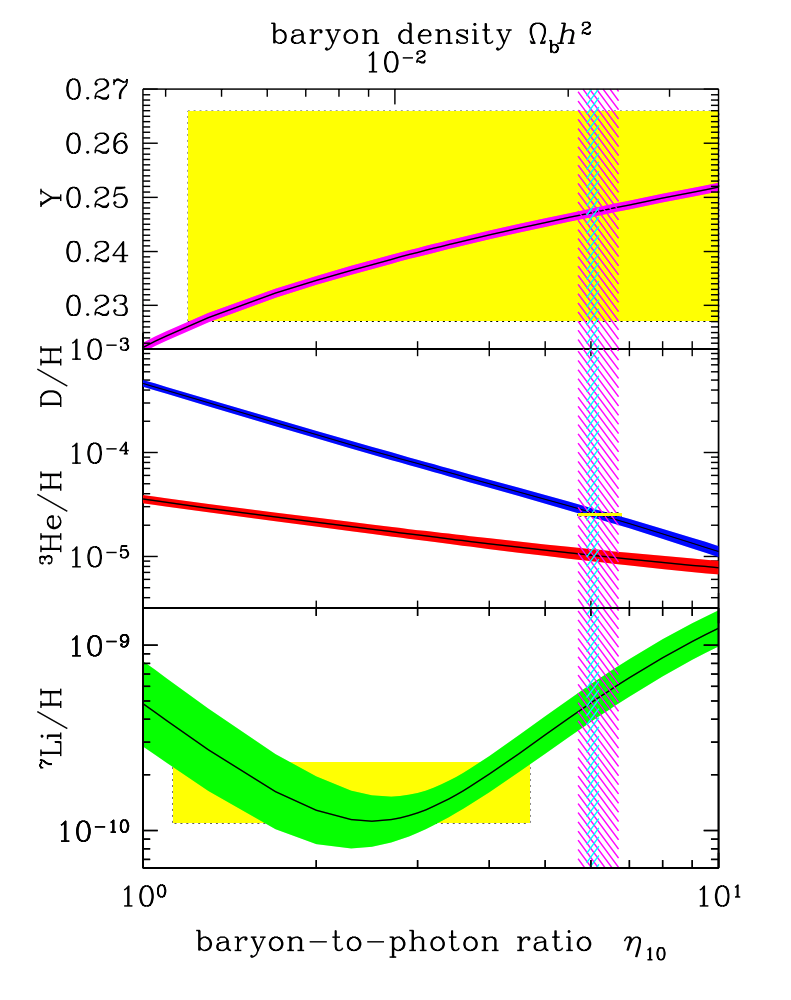
\includegraphics[width=0.6\linewidth]{abundances}
\caption{The abundances of the light elements as predicted by the standard model of BBN — the bands show the $95\%$ CL range. Boxes indicate the observed light element abundances. The narrow vertical band indicates the CMB measure of the cosmic baryon density, while the wider band indicates the BBN concordance range (both at $95\%$ CL) [taken from \citet{Fields:2014uja}].}\label{fig:abun}
\end{center}
\end{figure}


There are a vast array of different parameters and physics that go into computing the final abundances in Big Bang Nucleosynthesis. These include for example, the neutron-to-proton rate, $\Gamma_{n \rightarrow p}$, the strength of weak interaction, $G_F$, the Hubble constant $H(t)$, the baryon-to-photon ratio, $\eta$, etc. etc. We will focus on the particular parameters discussed in \citet{Fields:2014uja}. The relationship between these uncertainties and the predicted abundances is shown in Figure \ref{fig:abun}.

\begin{enumerate}
\item \textit{The baryon-to-photon ratio:} $\eta \equiv n_b/n_\gamma$ can explain the abundances in the standard model of BBN for $\eta_{10} \equiv \eta \times 10^{10}$ in the range $5.7 - 6.7$. If we view $n_\gamma$ as fixed by the CMB i.e. no error on $T_{\mathrm{CMB}} = 2.7255 \, \mathrm{K}$, then this can be translated into a bound on the allowed range for the baryon mass density today or the baryonic fraction of the critial density;
\begin{equation}
\rho_{b, 0} = (3.9 - 4.6) \times 10^{-31} \, \mathrm{g}\, \mathrm{cm}^{-3}, \quad \Omega_{b, 0} = \frac{\rho_b}{\rho_c} \simeq \frac{\eta_{10}h^{-2}}{274} = (0.021 - 0.025)h^{-2}.
\end{equation}
One can determine $\eta$ from the amplitudes of the acoustic peaks in the CMB
angular power spectrum, making it possible to compare two measures of $\eta$ using
very different physics, at two widely separated epochs. In the standard cosmology, there
is no change in $\eta$ between BBN and CMB decoupling, thus, a comparison of $\eta_{\mathrm{BBN}}$ and $\eta_{\mathrm{CMB}}$ is a key test. Agreement would endorse the standard picture, while disagreement could point to new physics during/between the BBN and CMB epochs.
\item \textit{The neutron lifetime:} this is most important for the determination of the helium abundance $Y_p$. Its value has recently been revised downwards to,
\begin{equation}
\tau_n = 880.0 \pm 0.9 \, \mathrm{s}.
\end{equation}
\end{enumerate}
The combination of these parameters with a Monte Carlo procedure gives the uncertainities illustrated in Figure \ref{fig:abun}. There has recently been a great deal of progress in the measuremnt of hydrogen and helium production as well as in the determination of cosmological parameters through Planck.


\subsection{Light Element Abundances}

BBN predicts that the abundances of the light elements (Deuterium, Helium-3, Helium-4, Lithium-7 etc.) are essentially fixed by $t \sim 180 \, \mathrm{s}$. On the other hand, abundances are observed at much latter epochs after stellar nucleosynthesis has commenced, producing the heavier elements C, N, O, Fe, etc. To measure primordial abundances, one then wants to look for low-metallicity environments where stellar nucleosynthesis has not distorted the quantities too significantly. In all of these measurements, the dominant limitation are the systematic uncertainties.

For deuterium, BBN is the only significant source, so any measurement provides a lower bound on its abundance. Measurements considering the lack of correlation between thevalue of $D/H$ and the metallicity/redshift/hydrogen column density is a standard way to infer that a measurement is indeed primordial. The highest precision measurement quoted in \citet{Fields:2014uja} is,
\begin{equation}
\mathrm{D}/\mathrm{H}|_p = (2.53 \pm 0.04)\times 10^{-5},
\end{equation}
where the subscript denotes the fact that this is primordial in nature. In addition to this, the primordial Helium abundance is best determined through recombination emission lines. Combined with data from the Sloan Digital Sky Survey of around 1000 galaxies, there is evidence that the helium abundance is positively correlated with metallicity. As such, extrapolation to the zero metallicity case is performed to infer the primordial abundance. The recommended Helium abundance in the PDG \cite{Fields:2014uja} is,
\begin{equation}
Y_p = 0.2465 \pm 0.0097.
\end{equation}
The same precision can not be found in Helium-3 measurements since the only data available is from high metallicity regions in the Milky Way. This makes inferring a primordial abundance difficult.


\subsection{The Lithium Abundance}


As you can see in Figure \ref{fig:abun}, theere is a discrepancy in the standard model between the allowed range of Lithium abundances and the parameters preferred by the CMB. From measurements in suitably metal-rich clusters, the recommended value is,
\begin{equation}
\mathrm{Li}/\mathrm{H}|_p = (1.6 \pm 0.3) \times 10^{-10}.
\end{equation}
Indeed, nuclear cross section data has recently increased the discrepancy to over $5\sigma$. There are a number of complicated new physics solutions proposed that include the injection of EM particles due to dark matter decays, or time variation in the fundamental constants. The other alternative of course is that there is some missing systematic error in the determination of the primordial measurement.


\newpage
\bibliography{main}
\end{document}